\chapter{Background and Literature Review}\label{chap:background}
\section{Simulation Environments}

As everyone is racing to develop the most innovative autonomous driving system, research is hindered by infrastructure costs and the logistical difficulties of training and testing systems in the physical world. Simulation has always been a central component of robotics development. This includes self-driving cars and various other applications. 

Among the many advantages of simulation environments is enabling engineers and researchers to perform faster research and development cycles. A new algorithm or a new sensor configuration can be implemented and tested with a minimum overhead. Algorithms and systems can be road-tested in a risk-free virtual environment where anything is possible and almost every real situation and corner-case can be considered. Another important advantage is system validation. 

After an autonomous agent software has been defined, exhaustive testing could be performed in the boundaries of a simulation environment in different scenarios, traffic patterns, weather conditions and many other environment variations, in addition to the simulation of dangerous situations. This allows intense testing of the autonomous car's system and its ability to react to abnormal conditions, without actually putting an individual in harm's way. This is critical to detect flaws in autonomous driving systems.

A physics simulator, that realistically represents physical aspects of an environment such as mass, forces, gravity and friction, is sufficient for some cases. However, for the applications of self-driving cars, especially for the perception task, a simulator platform must provide a photo-realistic representation of the environment, meaning that the simulated environment must actually look like the real world.

In this study, two simulation tools were used; the unity-based Udacity simulator, and the unreal-based CARLA simulator.
\pagebreak
\subsection{Udacity simulator}
Udacity, an on-line educational organization, has open-sourced its self-driving car simulator source code. This simulator was originally developed to help their Self-Driving Car Engineer Nanodegree students test and validate their projects. The simulator is based on Unity game engine. Given the popularity of Unity as a game development environment, and the open-source nature of the code, it is very convenient for modifications depending on the simulation need.The vehicle within the simulator can be manually driven to generate training data. 

Additionally, connection with a client (python or c++) can be established for an autonomous agent to take control of the vehicle. The simulation world is a racetrack that surrounds a lake and small hills, which is visually sufficient for a proof-of-concept, but not for final validation of algorithms.
\begin{figure}[ht]
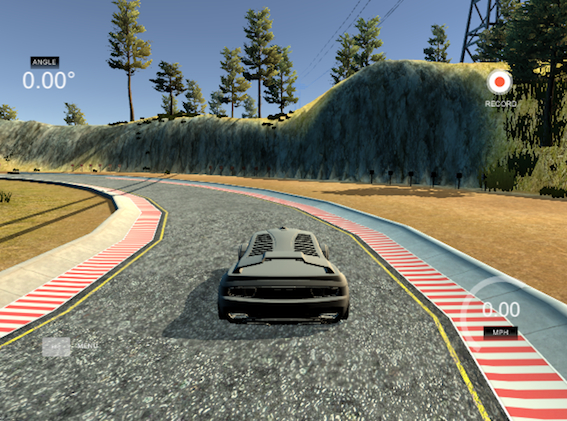
\includegraphics[width=\linewidth]{Figures/udacity_sim.png}
\centering
\caption{Udacity simulator racetrack environment}
\end{figure}
\pagebreak
\subsection{CARLA simulator}
CARLA is an open-source simulator for autonomous driving research. To reach such realistic graphics and visuals, the team behind the development of CARLA has used the unreal engine to base upon their simulator. Besides enabling the creation of worlds with photo-realistic roads, buildings and static environment components, the usage of the unreal game engine made it possible to add dynamic objects like cars and pedestrians to the scene.

In addition to a high-fidelity environment, a configurable sensors suite is available to the users, as well as control over weather conditions and time of the day. The result is a highly realistic environment, suitable for either testing any autonomous driving algorithm, or collecting data for artificial neural networks training.

Concerning interfaces with other software, the CARLA simulator can communicate through socket to any other software, either in the same machine or even over an Ethernet connection. Ground-truth data all traffic components, as well as vehicle state is provided by the simulator.

Other simulators like the Udacity simulator, TORCS, and many others lack pedestrians, intersections, cross traffic, traffic rules, and other complications that distinguish urban driving from track racing. Making CARLA the current best choice for training and validating systems that are expected/designed to operate in urban environments. Additionally, CARLA's photorealism allows for transfer learning, which is the process of training an artificial neural network inside the simulator, deploying it on a real vehicle, and fine tuning the network weights through further training on real collected data. This process decreases data collection time, decreases network training time, in addition to significantly increasing its performance.
\begin{figure}[ht]
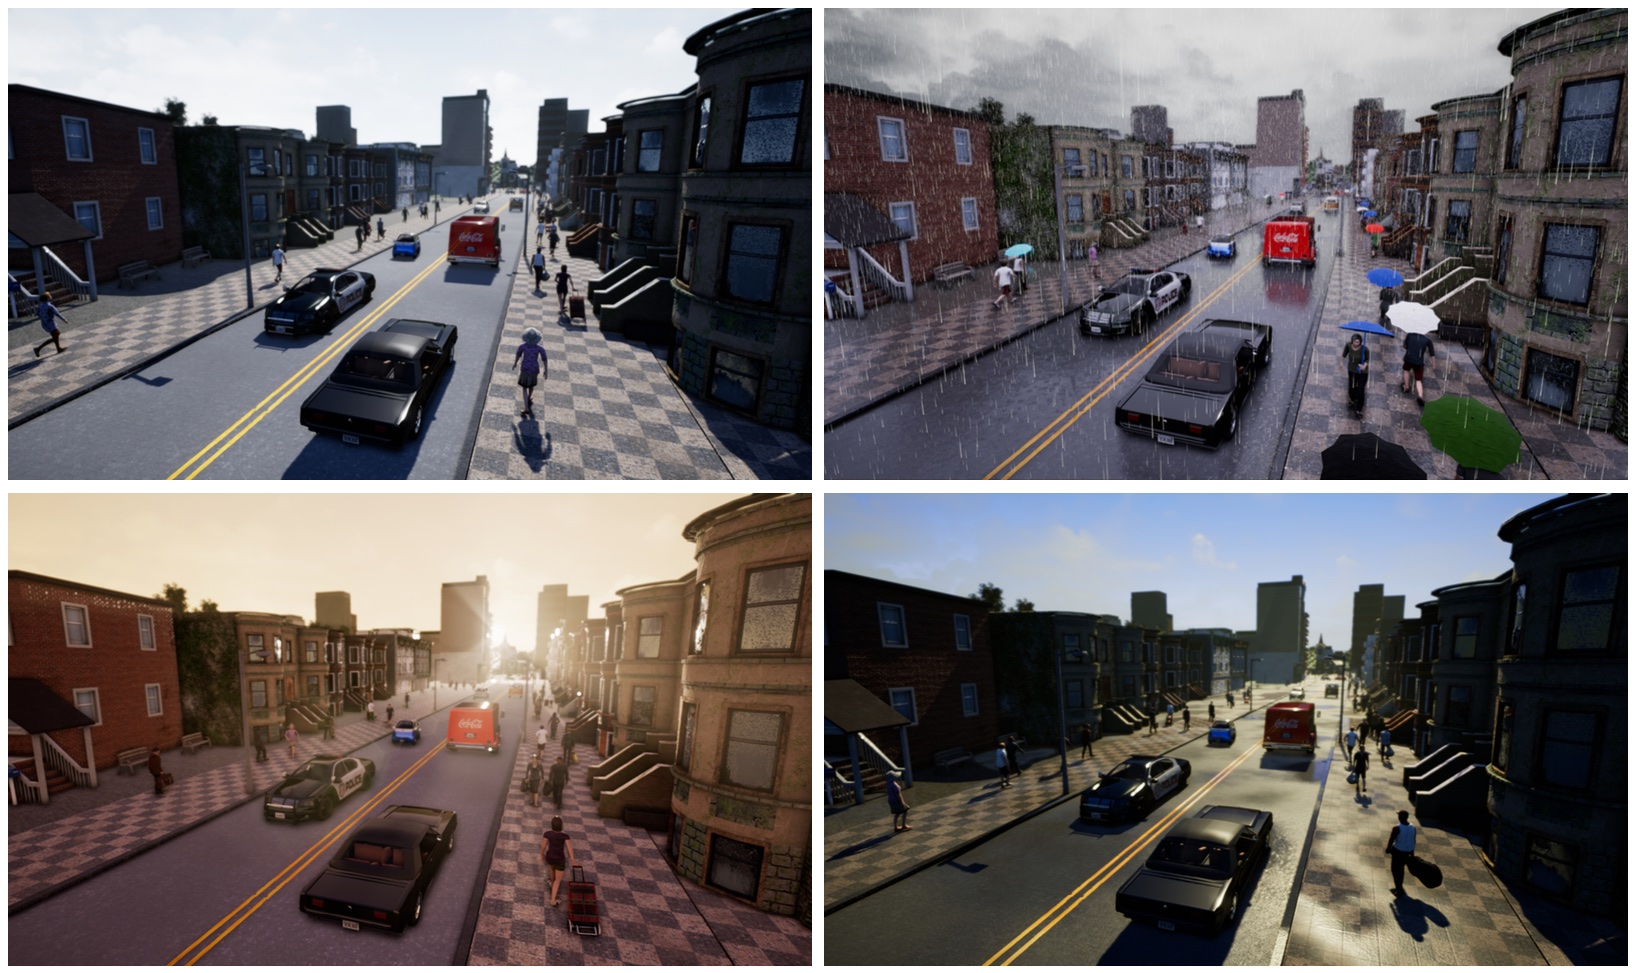
\includegraphics[width=\linewidth]{Figures/CARLA.jpg}
\centering
\caption{A scene within CARLA in different weather and light conditions}
\end{figure}
\pagebreak

\section{Driving data sets}
Machine learning and deep learning based algorithms have gained considerable popularity in the automated driving research field in the recent years. Given the fact that learning based algorithms thrive on data, enormous amount of driving data is in demand for training and testing purposes. This has made data collection on public roads and highways a valuable activity.

The process of data collection is usually executed by manually driving a vehicle. The driver is reactions are considered as the expert reaction when training or evaluating an algorithm. The vehicle is equipped with a set of sensors of different types, field of views, and mounting positions such as camera, LiDAR (Light Detection and Ranging), radar, ultrasonics, GPS, and IMU (inertial measurement unit). The sensor configuration (sensors type, count, mounting position) may vary depending on the use case for which the data is collected. The raw data received from different sensors is synchronized to fixed timestamps (frames) and logged on disk during the data collection process. Raw data produced by automotive sensors such as LiDARs and cameras is usually of large amounts, and of a high frequency nature. Accordingly, the expected size for the collected data can reach magnitudes of tens or even hundreds of gigabytes.

The data collection process is extremely time-consuming, especially on public roads and urban areas. To collect an amount of data that is sufficient to train a neural network, a fleet of vehicles and drivers is required. Additionally, the availability of large annotated datasets is a key to the successful use of deep learning in computer vision, however, it requires a large team of human annotators. Fortunately, there exists a lot of driving datasets collected by institutes and companies that are heavily investing in the self-driving car domain. With the increasing popularity of open-source development, many of those companies and institutes have provided open access to such datasets, along with detailed documentation and user guides. However, driving datasets are different when it comes to sensor setup, data format and driving conditions, making the choice of the appropriate data set a challenging task.

Many of the available datasets provide a benchmarking framework. This provides researchers with a performance indicator of the implemented algorithms, which compares the algorithm's output to the ground truth data included in the dataset.
\pagebreak
\subsection{The KITTI data set}
\begin{wrapfigure}{r}{6.5cm}
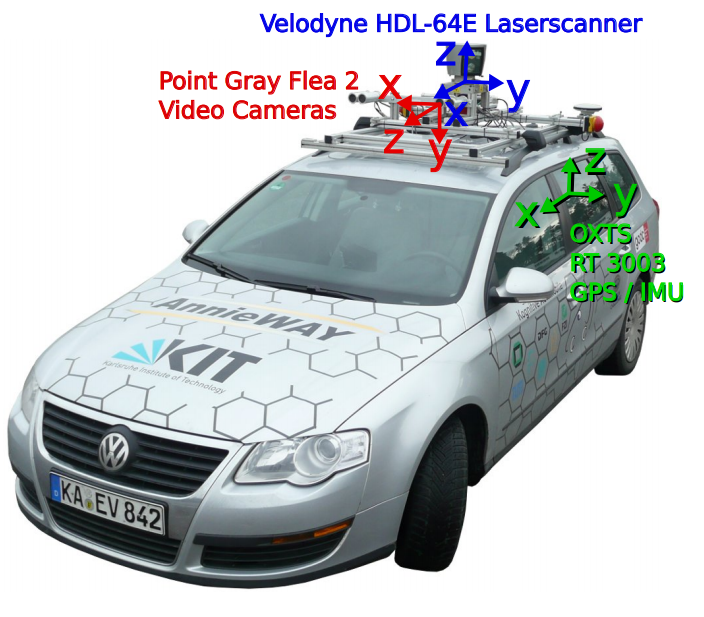
\includegraphics[width=\linewidth]{Figures/KITTI_platform.png}
\centering
\caption{KITTI recording platform \cite{kitti}}
\end{wrapfigure} 
% \begin{figure}[ht]
% 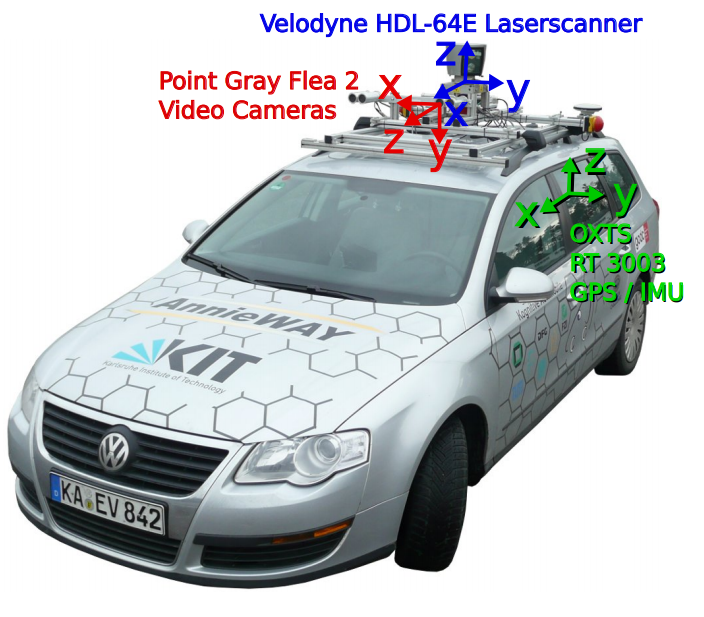
\includegraphics[width=0.6\linewidth]{Figures/KITTI_platform.png}
% \centering
% \caption{KITTI recording platform \cite{kitti}}
% \end{figure}

% \begin{figure*}[ht!]
% \centering
% \begin{subfigure}[t]{0.5\textwidth}
% \centering
% 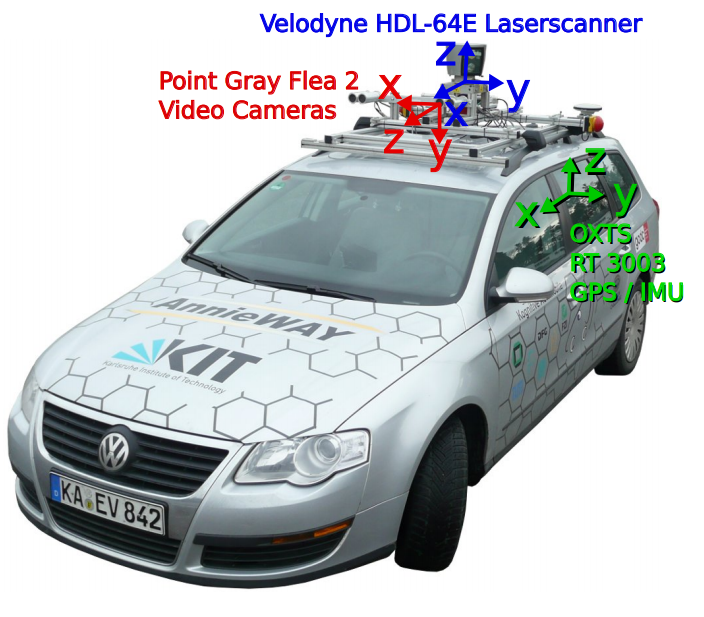
\includegraphics[width=0.6\linewidth]{Figures/KITTI_platform.png}
% \caption{Recording platform}
% \end{subfigure}%
% ~ 
% \begin{subfigure}[t]{0.5\textwidth}
% \centering
% 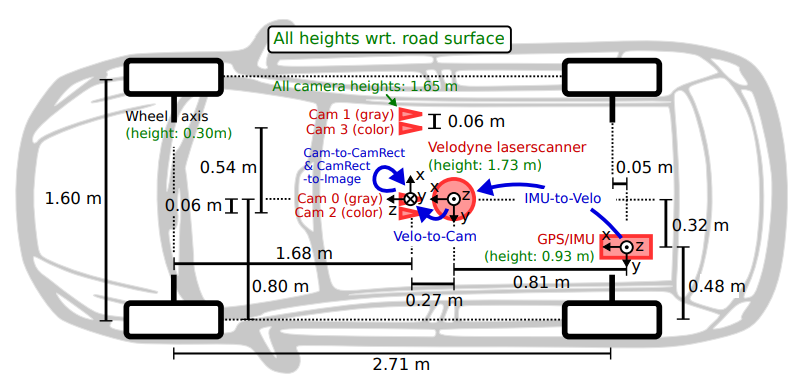
\includegraphics[width=1.2\linewidth]{Figures/KITTI_sensors.png}
% \caption{Sensor configuration}
% \end{subfigure}
% \caption{KITTI platform and sensor configuration \cite{kitti}}
% \end{figure*}

KITTI is the outcome of the collaboration between the Department of Measurement and Control Systems in Karlsruhe Institute of Technology (KIT, Karlsruhe, Germany) and Toyota Technological Institute (TTI, Chicago, USA).   

\subsubsection{Sensor setup}
The Recording Platform is a VW Passat station wagon. The vehicle is equipped with a variety of sensor modalities including four high resolution video cameras (two color and two grayscale cameras), a rotating
3D velodyne laser scanner and a combined GPS/IMU inertial navigation and localization system. The coordinate transformations between different sensor frames are also provided as shown in Figure \ref{kitti_sensors}. Data capturing is done by driving around the city of Karlsruhe. This includes highways and rural areas.

\begin{figure}[ht]
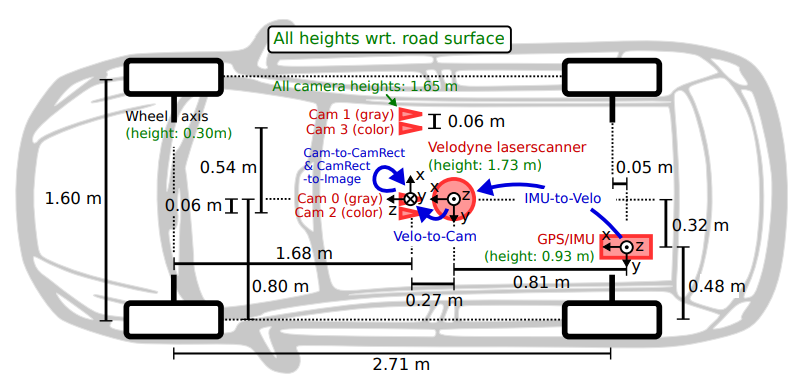
\includegraphics[width=\linewidth]{Figures/KITTI_sensors.png}
\centering
\caption{KITTI platform sensor configuration \cite{kitti}}
\label{kitti_sensors}
\end{figure}

\subsubsection{KITTI Road and Lane estimation benchmark}
Although most vehicles are currently equipped with lane detection systems, such algorithms can only function on well-marked roads and highways. However, in urban and city environments it can be very challenging to boundaries of unmarked or weakly marked roads and lanes due to the high variations in road types and profiles, as well as illumination conditions.

The KITTI data set provides a benchmark for road and lane estimation. The benchmark consists of 289 training images and 290 test images. Road scenes are categorized into three types as shown in Figures \ref{kitti_raw_road} and \ref{kitti_labeled_road}:
\begin{itemize}
\item UU - urban unmarked
\item UM - urban marked
\item UMM - urban multiple marked lanes
\end{itemize}


Given the fact that vehicle control happens in the 2D Bird’s Eye View (BEV) space, detection results are required to be represented in this very same space. This is crucial for a meaningful evaluation since pixel-level performance is of limited value for vehicle control. Classical pixel-level metrics in perspective and BEV space are used to evaluate state-of-the-art road detection algorithms.

\begin{figure}[ht]
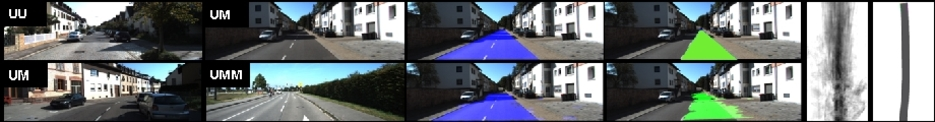
\includegraphics[trim={0cm 0 19cm 0cm},clip,width=\linewidth]{Figures/KITTI_road.jpg}
\centering
\caption{KITTI road and lane estimation example raw frames \cite{kitti_road}}
\label{kitti_raw_road}
\end{figure}

\begin{figure}[ht]
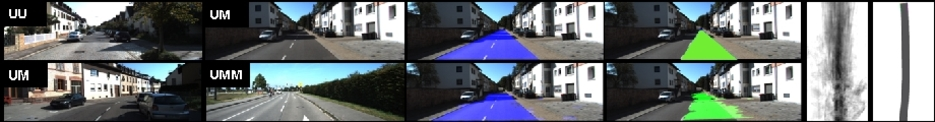
\includegraphics[trim={15cm 0cm 0cm 0cm},clip,width=\linewidth]{Figures/KITTI_road.jpg}
\centering
\caption{KITTI road and lane estimation example labeled frames \cite{kitti_road}}
\label{kitti_labeled_road}
\end{figure}

\subsection{GTI vehicle image database}
The Grupo de Tratamiento de Imágenes (GTI) vehicle image dataset is developed by Universidad Politécnica de Madrid (UPM) to evaluate algorithms that are targeting the vision-based vehicle classification task. Images are extracted from video sequences acquired with a forward looking camera mounted on a vehicle.

\begin{figure}[ht]
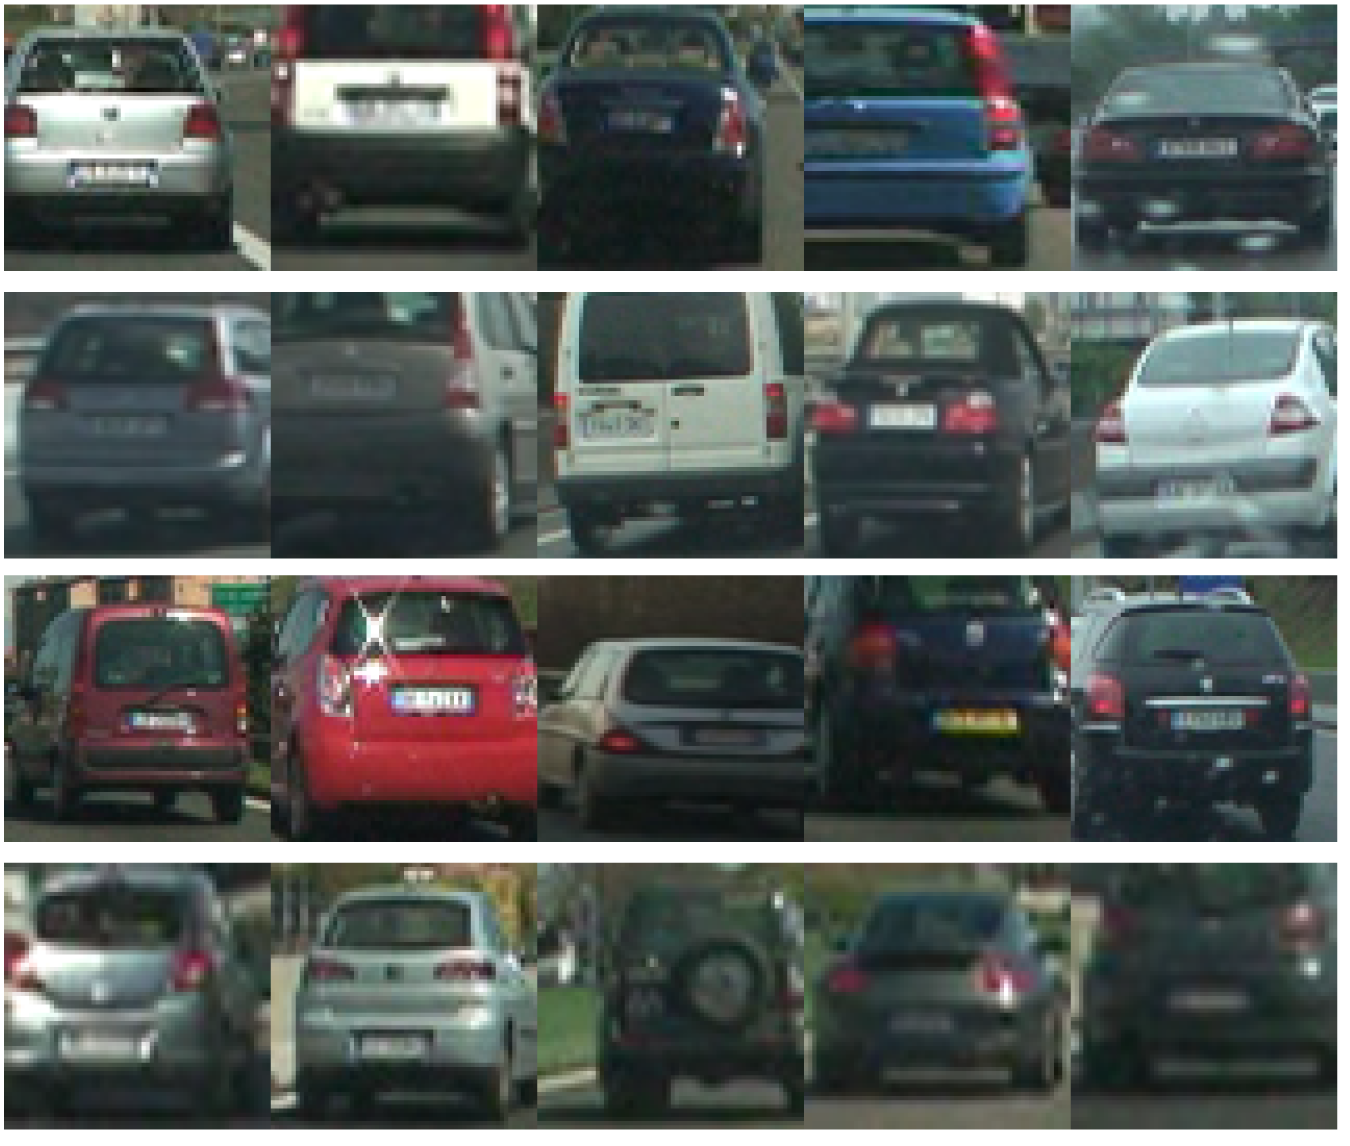
\includegraphics[trim={0cm 0cm 0cm 0cm},clip,width=\linewidth]{Figures/GTI.png}
\centering
\caption{GTI vehicle image database example frames \cite{gti}}
\label{gti}
\end{figure}

The database contains 3425 images of vehicle rears taken from different points of view, and 3900 images extracted from road sequences not containing vehicles. Images are selected to maximize the representativity of the vehicle class, which involves a naturally high variability. The position of the vehicle relative to the camera is a relevant factor affecting the appearance of the vehicle rear. Accordingly, images are categorized into four types based on the pose:

\begin{itemize}
\item middle/close range in front of the camera
\item middle/close range in the left
\item close/middle range in the right
\item far range
\end{itemize}

Additionally, images are deliberately extracted with an imperfect fit to the actual vehicle contour which results in the inclusion of some background areas in the image, or even partial inclusion of the vehicle. This is to ensure the robustness of the classifier in question. The images have 64x64 and are cropped from sequences of 360x256 pixels recorded in highways of Madrid, Brussels and Turin \cite{gti}.

\subsection{Udacity data set}
\begin{figure}[ht]
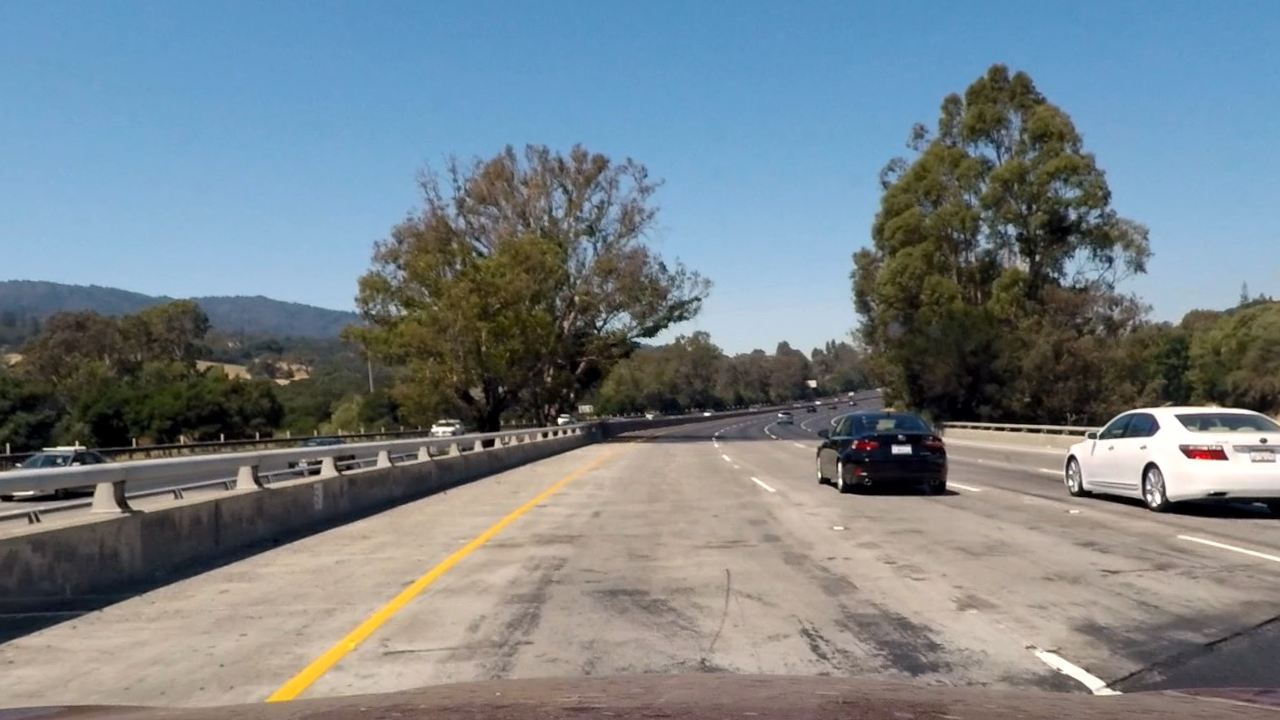
\includegraphics[trim={0cm 0cm 0cm 0cm},clip,width=\linewidth]{Figures/test1.jpg}
\centering
\caption{Udacity driving dataset example frame}
\label{udacity_data}
\end{figure}
As part of their self-driving car nanodegree program, Udacity had to tackle their own self-driving car project. In an attempt to democratize education, they have created their self-driving car platform with Open source code, written by hundreds of students from across the globe.

To build such open source project, the platform was built on a 2016 Lincoln MKZ. Two Velodyne VLP-16 LiDARs, 1 Delphi radar, 3 Point Grey Blackfly cameras, an Xsens IMU, an ECU, a power distribution system were installed. The platform was configured to use Robot Operating System (ROS) as its middle-ware.

A dataset was collected using the aforementioned platform that consists of PNG images from the center camera only. In addition to a log file with various vehicle signals including the steering angle. All resources provided by Udacity are open-source. They have also posted several challenges to encourage the self-driving car community to develop new systems based on Udacity's platform.


\section{Machine Learning and Deep Learning}
The science of machine learning is heavily based on the backpropagation process. Backpropagation is a way of computing gradients of expressions through recursive application of chain rule. Understanding backpropagation is essential for understanding, developing, designing and debugging Neural Networks.

\subsection{Gradient of simple expressions}

If a simple multiplication function of two numbers is considered, \(f(x,y)=xy\). Deriving the partial derivative for either input can be done using simple calculus:
\begin{equation}
f(x,y) = x y \hspace{0.5in} \rightarrow \hspace{0.5in} \frac{\partial f}{\partial x} = y \hspace{0.5in} \frac{\partial f}{\partial y} = x
\label{multiplication_deriv}
\end{equation}

Derivatives indicate the rate of change of a function with respect to a variable surrounding an infinitesimally small region near a particular point:
\begin{equation}
\frac{df(x)}{dx} = \lim_{h\ \to 0} \frac{f(x + h) - f(x)}{h}
\end{equation}

Unlike the division sign on the right-hand side, the division sign on the left-hand side is not a division, but rather a notation that indicates that the operator \(\frac{d}{dx}\) is being applied to the function \(f\), and returns a different function that is the derivative of \(f\). The expression above states that when h is a very small value, the function can be well-approximated by a straight line with the derivative representing its slope. Accordingly, the derivative on each variable represents the sensitivity of the expression on the value of this variable.

Similarly, the derivatives of the addition operation can also be derived:
\begin{equation}
f(x,y) = x + y \hspace{0.5in} \rightarrow \hspace{0.5in} \frac{\partial f}{\partial x} = 1 \hspace{0.5in} \frac{\partial f}{\partial y} = 1
\label{add_deriv}
\end{equation}

It is noted that the derivative on both x,y is independent of what the actual values of x,y are. Unlike the multiplication function, increasing either x,y would increase the output of the addition function regardless of the value of the other.


The gradient of a function \(f(x,y)\) is represented by a vector of the partial derivatives \(\nabla f\), where \(\nabla f = [\frac{\partial f}{\partial x}, \frac{\partial f}{\partial y}] = [y, x]\)

\subsection{Gradient of complex expressions by the chain rule}
A different approach is taken to calculate the derivative vector for more complicated expressions that involve multiple composed functions, such as:
\begin{equation}
f(x,y,z)=(x+y)z
\label{complex}
\end{equation}
This expression can be decomposed into two simpler expressions: 
\begin{equation}
q=x+y \hspace{0.25in},\hspace{0.25in} f=qz
\end{equation}
The derivatives of both expressions can be computed separately as stated in the previous section. Since \(f\) is the multiplication of \(q\) and \(z\), therefore:
\begin{equation}
\frac{\partial f}{\partial q} = z \hspace{0.25in},\hspace{0.25in} \frac{\partial f}{\partial z} = q
\end{equation}

Since \(q\) is the addition of \(x\) and \(y\), therefore:
\begin{equation}
\frac{\partial q}{\partial x} = \frac{\partial q}{\partial y} = 1
\end{equation}
Based on the chain rule, multiplication is the correct way to chain these gradient expressions together. Accordingly, \(\frac{\partial f}{\partial x}\) can be calculated as:
\begin{equation}
\frac{\partial f}{\partial x} = \frac{\partial f}{\partial q} \frac{\partial q}{\partial x}
\label{partial_x}
\end{equation}
\begin{figure}[ht]
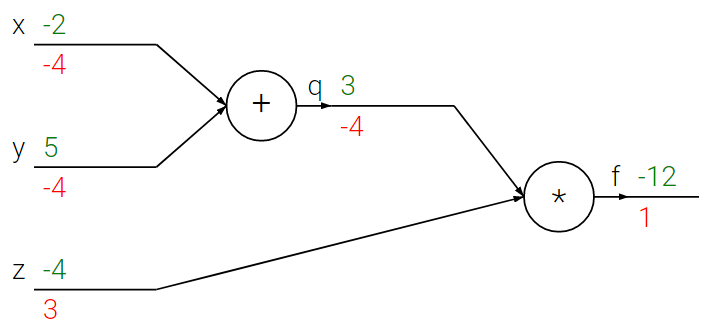
\includegraphics[trim={0cm 0cm 0cm 0cm},clip,width=0.75\linewidth]{Figures/grad_1.png}
\centering
\caption{A visual representation of equations \ref{complex}-\ref{partial_x}. Output values are computed from inputs (green).Backpropagation is used to recursively apply the chain rule to compute the gradients (red), starting at the end and passing back to the inputs.}
\label{grad_1}
\end{figure}


\subsection{Backpropagation}
Backpropagation is a local process. For a specific function, the output values and the local gradients of its inputs with respects to its outputs can be calculated once it receives an input. This can be independently done for each single function without prior knowledge of other functions the are the source of its inputs or the destination for its outputs. As the forward pass is complete, the gradient of each function's output value on the final output will be known. Chain rule says that the gradient of a function's output value on the final output should be multiplied  into every gradient that is normally computed for all of the function inputs. Accordingly, backpropagation can be considered as a means of communicating between different functions through the gradient signal, providing each function with the numerical measure of how effective is its output on the final output. \cite{backprop}

Any differentiable function can be considered as a gate. A single gate can be decomposed into multiple gates if applicable, and multiple gates can be grouped into a single gate.
\begin{equation}
f(w,x) = \frac{1}{1+e^{-(w_0x_0 + w_1x_1 + w_2)}}
\label{sigmoid}
\end{equation}
Equation \ref{sigmoid} describes a 2-dimensional neuron (gate) with inputs \(x\) and weights \(w\), and uses the sigmoid function as its activation function. For simplicity, this neuron can be broken down to multiple simple gates represented by Equations \ref{add_deriv} and \ref{multiplication_deriv} along with the equations below:
\begin{equation}
f(x) = \frac{1}{x} 
\hspace{1in} \rightarrow \hspace{1in} 
\frac{df}{dx} = -1/x^2 
\end{equation}
\begin{equation}
f_c(x) = c + x
\hspace{1in} \rightarrow \hspace{1in} 
\frac{df}{dx} = 1 
\end{equation}
\begin{equation}
f(x) = e^x
\hspace{1in} \rightarrow \hspace{1in} 
\frac{df}{dx} = e^x
\end{equation}
\begin{equation}
f_a(x) = ax
\hspace{1in} \rightarrow \hspace{1in} 
\frac{df}{dx} = a
\end{equation}
The functions \(f_c,f_a\) are simple addition and multiplication function, that translate the input by a constant of c and scale the input by a constant of a, respectively. However, both functions are treated as special functions since the gradients for the constants \(c,a\) are of interest. 

\begin{figure}[!ht]
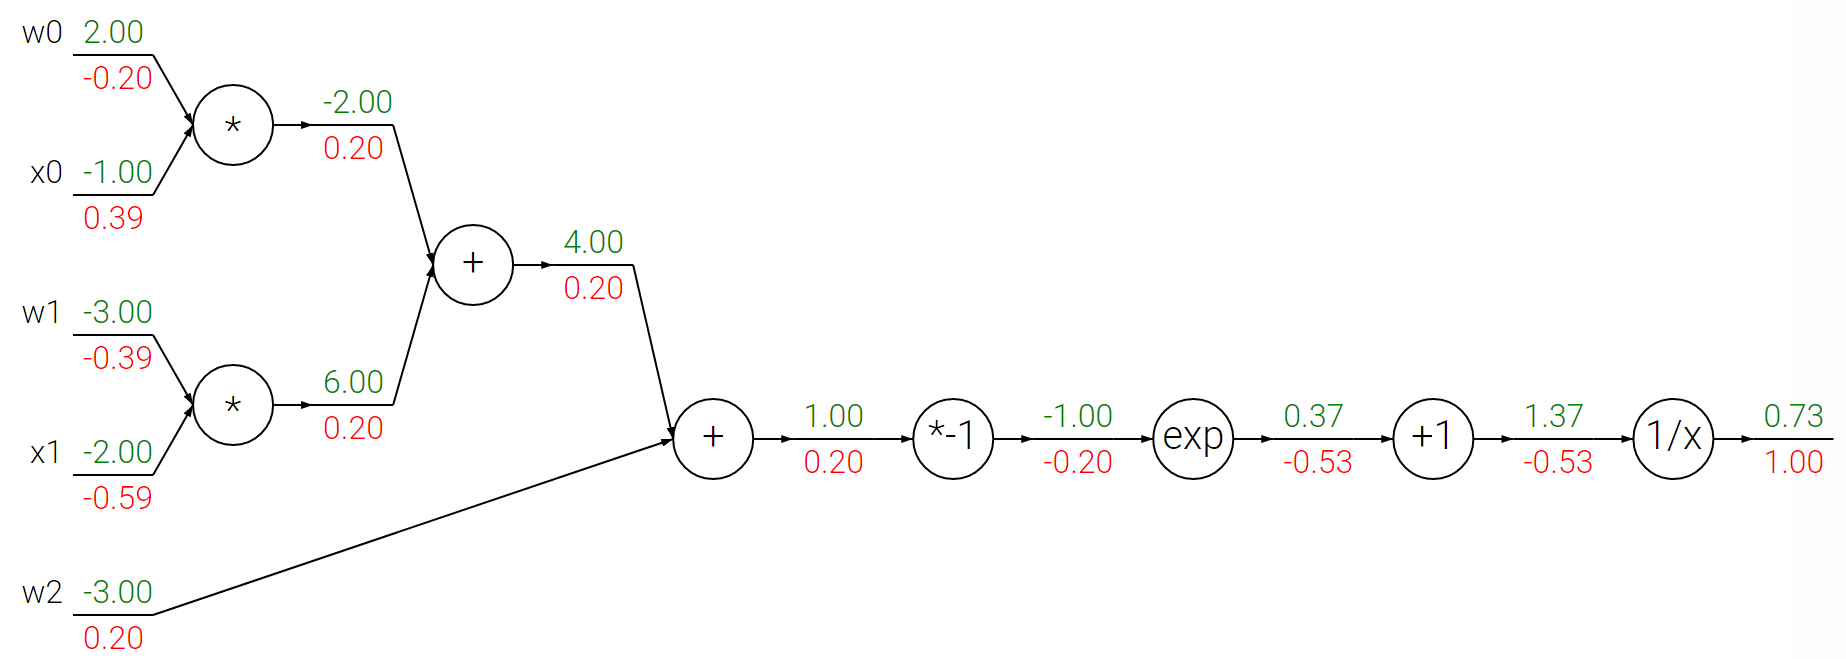
\includegraphics[trim={0cm 0cm 0cm 0cm},clip,width=\linewidth]{Figures/sigmoid.png}
\centering
\caption{A circuit representing a 2D neuron with a sigmoid function as its activation function. \([x0,x1]\) are the inputs  and \([w0,w1,w2]\) are the learn-able weights of the neuron}
\label{signmoid_circuit}
\end{figure}

The full sigmoid function can be represented by Figure \ref{signmoid_circuit} after decomposing it to simpler gates. It is observed that the result of the dot product between the vectors \(w,x\) is fed into a long chain of gates. The function that these gates implement is the sigmoid function \(\sigma(x)\).

\begin{equation}
\sigma(x) = \frac{1}{1+e^{-x}} \\\\
\rightarrow \hspace{0.3in} \frac{d\sigma(x)}{dx} = \frac{e^{-x}}{(1+e^{-x})^2} = \left( \frac{1 + e^{-x} - 1}{1 + e^{-x}} \right) \left( \frac{1}{1+e^{-x}} \right) 
= \left( 1 - \sigma(x) \right) \sigma(x)
\label{sig_deriv}
\end{equation}
Equation \ref{sig_deriv} shows that the derivative of the sigmoid function can be derived and simplified to be a function of the sigmoid itself. In other words, once the forward pass is executed, and \(\sigma(x)\) is calculated for a given \(x\) value, the local gradient can simply be calculated as \(( 1 - \sigma(x)) \sigma(x)\). For example, for an input of \(1.0\), the output would be \(0.73\), and accordingly the local gradient can be calculated as \((1 - 0.73) * 0.73 \approx 0.2\). This shows the benefit of grouping a chain of gates into a single gate.

\subsection{Neurons}
The modeling of biological neural systems has originally been the primary goal and inspiration of Neural Networks. Nonetheless, with the advances in research it has diverged to become a matter of engineering and a science of designing systems that are intelligent enough to solve human tasks.



A neuron is the basic computational unit of the brain. The human nervous system contains approximately 86 billion neurons that are connected with approximately \(10^{14} - 10^{15}\) synapses. Each neuron receives input signals from its dendrites (multiple) and produces output signals along its (single) axon. The axon eventually branches out and connects via synapses to dendrites of other neurons.

\subsubsection{Artificial Neurons}
\begin{figure*}[ht!]
\centering
\begin{subfigure}[t]{0.5\textwidth}
\centering
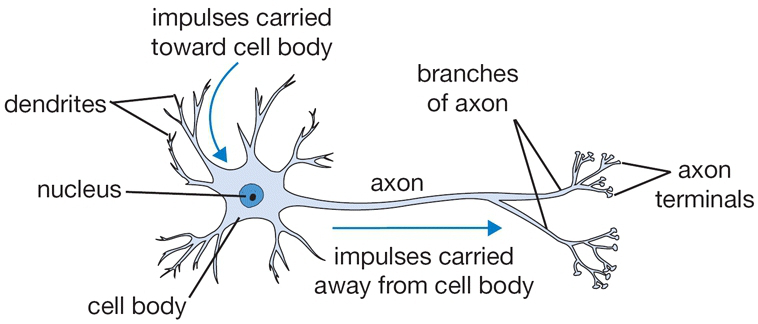
\includegraphics[width=\linewidth]{Figures/neuron.png}
\caption{Biological brain neuron}
\end{subfigure}%
~ 
\begin{subfigure}[t]{0.5\textwidth}
\centering
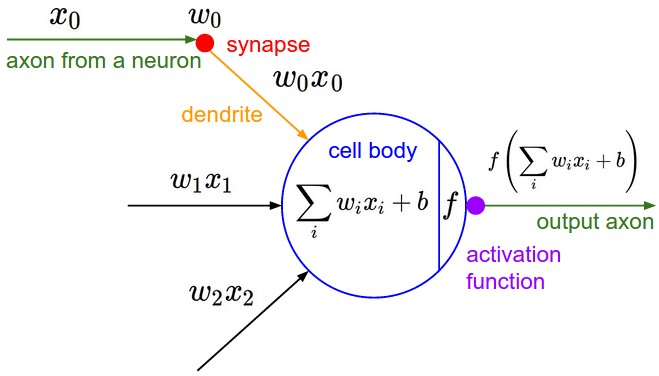
\includegraphics[width=\linewidth]{Figures/neuron_model.jpeg}
\caption{Artificial neuron}
\end{subfigure}
\caption{Comparison between Biological neuron and artificial neuron}
\label{neurons}
\end{figure*}
Figure \ref{neurons} shows a comparison between a biological neuron and a common mathematical model of the artificial neuron. 

In the computational model of a neuron, the signals that travel along the axons \((x0)\) interact multiplicatively \((w0x0)\) with the dendrites of the other neuron based on the synaptic strength at that synapse \((w0)\). The synaptic strengths are represented by the weights \(w\). The weights for each neuron are learn-able and control the strength of influence of one neuron on another. Such influence can be excitatory (positive weight) or inhibitory (negative weight). 
\subsubsection{Activation Functions}
In the aforementioned simplified model, the neuron's inputs are multiplied by their respective weights, and are then carried by the neuron's dendrites to the cell body where they are all added together. Additionally, a bias value is added to the summation of all weighted inputs. If the final sum is then passed to an activation gate which decides if the neuron should fire, sending the output spike along its axon. 

In the computational model, temporal differences between activations are ignored. A common choice of the activation function is the sigmoid function \(\sigma\), since it takes as an input a real-number, which is the signal strength after the weighted sum and converts it to a number that ranges between 0 and 1. Another common activation function is the \(\tanh\) function takes as an input a real-number, which is the signal strength after the weighted sum and converts it to a number that ranges between -1 and 1. Both functions are shown in Figure \ref{activation}.

\begin{figure*}[ht!]
\centering
\begin{subfigure}[t]{0.5\textwidth}
\centering
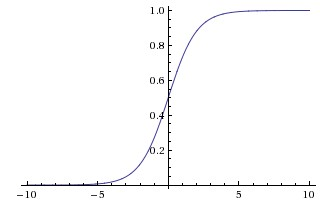
\includegraphics[width=\linewidth]{Figures/sigmoid.jpeg}
\caption{Sigmoid activation function}
\end{subfigure}%
~ 
\begin{subfigure}[t]{0.5\textwidth}
\centering
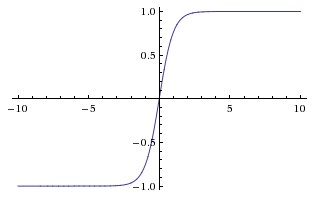
\includegraphics[width=\linewidth]{Figures/tanh.jpeg}
\caption{Artificial neuron}
\end{subfigure}
\caption{Commonly used activation functions}
\label{activation}
\end{figure*}

\subsection{Fully-Connected Neural Networks (FCNs)}
A collection of neurons that are connected in an acyclic graph is referred to as a neural network. In such a network the output of a neuron can become an input to another neuron. Neural network models are usually designed in layers of neurons. Cycles are not allowed since that would imply an infinite loop in the forward pass of a network. The most common layer type is the fully-connected layer in which neurons between two adjacent layers are fully pairwise connected, however, neurons within a single layer share no connections. Neural network are thought of as \textbf{Universal Function Approximators}. Given enough data, a network can approximate a complex function to simpler neurons.
\begin{figure}[ht]
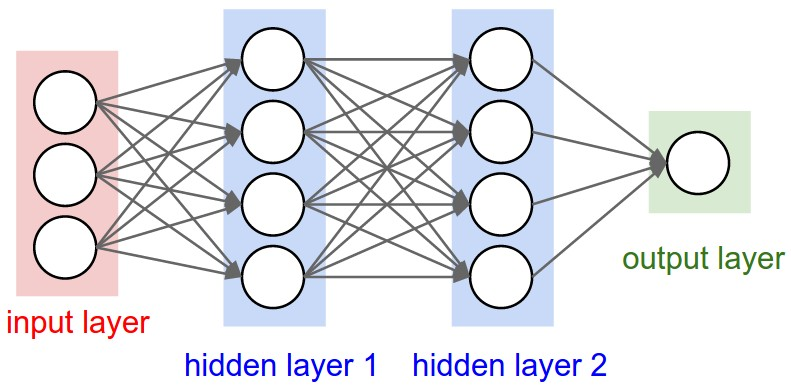
\includegraphics[trim={0cm 0cm 0cm 0cm},clip,width=\linewidth]{Figures/neural_net2.jpeg}
\centering
\caption{A three layer fully-connected neural network.}
\label{network_architecture}
\end{figure}
\subsubsection{Network Architectures}
Figure \ref{network_architecture} shows a three layer neural network (two hidden layers and one output layer). Synapses, which are connections between neurons, are present between neurons across layers, but not within a layer.

Unlike all layers in a Neural Network, the output layer neurons most commonly do not have an activation function. For example, in a classification problem, the output layer usually represents the probability of the input classification, with each neuron output representing a class. 

The number of neurons and the number of parameters are the commonly used metrics for measuring the size of a neural network. Excluding the input layer, the network represented in Figure \ref{network_architecture} has \(4 + 4 + 1 = 9\) neurons, \([3 * 4] + [4 * 4] + [4 * 1] = 12 + 16 + 4 = 32\) weights and \(4 + 4 + 1 = 9\) biases, for a total of \(41\) learn-able parameters. There are special cases where some parameters are learn-able and some are not.
\subsubsection{Network Capacity}
As the size and number of layers in a Neural Network increases, the capacity of the network increases. A network's capacity is the space of representable functions. This is due to the fact that more neurons can collaborate to express many different functions. 
\begin{figure}[ht!]
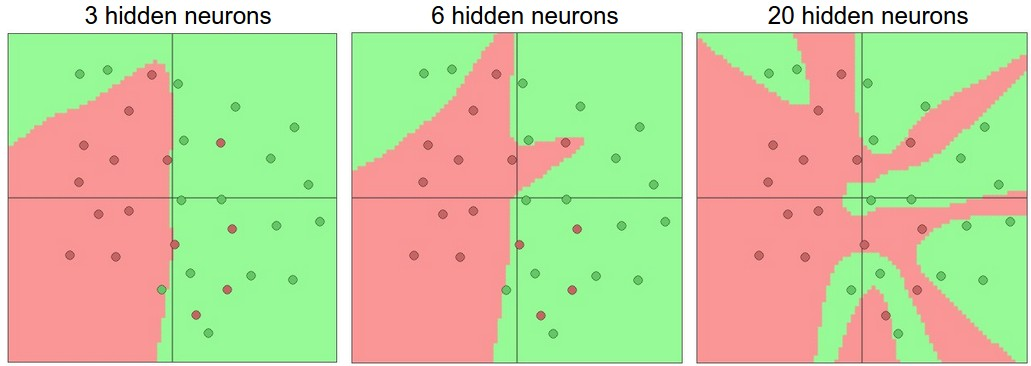
\includegraphics[trim={0cm 0cm 0cm 0cm},clip,width=\linewidth]{Figures/layer_sizes.jpeg}
\centering
\caption{A three layer fully-connected neural network.}
\label{network_capacity}
\end{figure}

Figure \ref{network_capacity} shows a binary classification problem in two dimensions. The data are shown as circles colored by their class. Three separate neural network models are trained to classify the data. All three network architectures have one hidden layer while varying the number of neurons. The decision regions by a trained neural network are shown by color underneath the data points. This shows that as the number of neurons increases, its ability to express more complicated functions also increases. However, as useful as this can be when classifying complicated data, a complex network is more likely to over-fit the training data.

Over-fitting occurs when a high capacity model accurately fits the data that it is affected by the noise instead of the underlying pattern. Considering the aforementioned example, the model with 3 hidden neurons only has the representational power to classify the data in broad strokes. It classifies the whole space into two decision regions, and considers the few red points inside the green region as \textbf{outliers} (noise). On the other hand, the model with 20 hidden neurons classifies the space into many disjoint red and green decision regions and is able to fit all the training data. This leads to better accuracy on the training data set at the cost of poor \textbf{generalization} on the test set. 
\subsubsection{Over-fitting}
However, in practice, it is always better to use methods such as L2 regularization, dropout, input noise, and others to control over-fitting rather than decreasing the number of neurons. Regularization strength is the preferred way to control the over-fitting of a neural network.

\begin{figure}[ht!]
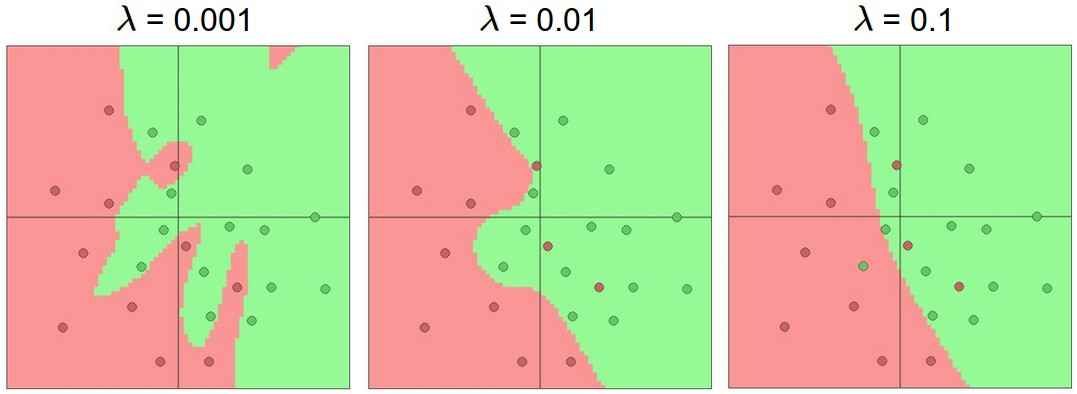
\includegraphics[trim={0cm 0cm 0cm 0cm},clip,width=\linewidth]{Figures/reg_strengths.jpeg}
\centering
\caption{The effects of regularization strength}
\label{reg_strength}
\end{figure}

All three neural networks shown in Figure \ref{reg_strength} have 20 hidden neurons. It is observed that changing the regularization strength affects the smoothness of the network's final decision regions. Higher regularization strength allows for better generalization at the cost of a decreased training set accuracy. The correct balance should be reached based on the application, data exploration, and exploitation.

Generally, smaller networks should not always be the solution to over-fitting. Instead, a neural network should be as big as the computational budget allows, with the use of regularization techniques to control over-fitting.

FCNs have some serious disadvantages when dealing with images. For example, an RGB image of size \((200,200)\) would lead to neurons that have \(200*200*3 = 120,000\) weights. Additionally, since a network would need several neurons to execute any task, the number of weights would be multiplied by the number of neurons. This will eventually result in a huge number of hyper-parameters which will inevitably cause over-fitting. The solution to such problem lies in the concept of Convolution which is inherited from the science of image processing and computer vision.

\subsection{Convolution Neural Networks (CNNs/ConvNets)}
Convolution Neural Networks are very similar to the previously mentioned fully-connected Neural Networks from the previous section. They are similarly composed of neurons that have learn-able weights and biases. For each neuron the dot product of the inputs is calculated and is optionally followed non-linear activation function. Similar to FCNs, the whole network expresses a single differentiable score function with the raw image pixels on one end, and class scores at the other. Backpropagation is applied with a loss function on the last layer to train the weights and biases.

\begin{figure}[ht]
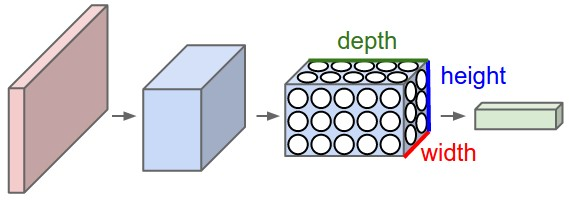
\includegraphics[trim={0cm 0cm 0cm 0cm},clip,width=\linewidth]{Figures/cnn.jpeg}
\centering
\caption{Convolution Neural Network architecture}
\label{cnn}
\end{figure}

In contrast to FCNs, CNN architectures make the explicit assumption that the inputs are images. This allows the encoding of certain properties into the architecture which makes the forward function more efficient to implement, in addition to the reduction of parameters in the network.

Unlike a Fully-Connected Neural Networks, neurons in a layers of a Convolution Neural Network are arranged in 3 dimensions: width, height, depth, with depth referring to the third dimension of an activation volume, which, for an RGB image, is the 3 channels as shown in Figure \ref{cnn}. For example, for an RGB input image of size \((32,32)\), the input activation volume has dimensions \((32,32,3)\) (width, height, depth respectively). Instead of connecting all of the neurons in a fully-connected manner, neurons in a layer will only be connected to a small region of the layer preceding it. Accordingly, the final output layer would have dimensions \((1,1,10)\). The length of the output vector is equal to the number of desired classes that are expected from the network to classify.

\subsubsection{CNN Layers}
Similar to the FCN, a simple CNN is a sequence of layers. Each Layer accepts an input 3D volume and transforms it to an output 3D volume through a differentiable function. Three main types of layers are used to build a CNN architectures: 
\begin{itemize}
\item Convolution Layer
\item Pooling Layer
\item Fully-Connected Layer
\end{itemize}
\subsubsection{Convolution Layer}
\begin{figure}[ht]
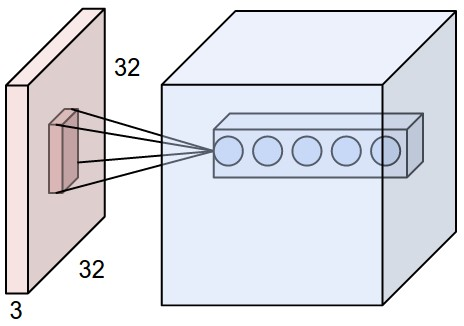
\includegraphics[trim={0cm 0cm 0cm 0cm},clip,width=0.7\linewidth]{Figures/depthcol.jpeg}
\centering
\caption{A visualization of the convolution process}
\label{conv}
\end{figure}
From the image processing perspective, a convolution layer’s parameters are a set of learn-able filters. Every filter extends through the full depth of the input volume, but is spatially small along width and height. A typical filter on a first layer of a CNN which accepts as input an RGB image would have the dimensions \((5,5,3)\). During the forward pass, each filter passes across the width and height of the input volume as shown in Figure \ref{conv}. The dot product between the filter parameters (weights) and the input at any position is computed. This will produce a 2-dimensional activation map representing the responses of that filter at every spatial position. Accordingly, the network will learn to see visual features in an image. Such visual features can include an edge of some orientation or a patch of a specific color on the first layer. Higher layers of the network can eventually learn to detect specific patterns in an image. Individual 2-dimensional activation maps produced by every filter in the convolution layer will be stacked along the depth dimension, producing the output volume.

Every entry in the 3D output volume can also be interpreted as an output of a neuron that focuses on a small region in the input image. This neuron shares parameters with all neurons that are in close spatial proximity in all four directions, since these numbers are all the result of applying the same filter on the input image in a convolution. 

\subsubsection{Pooling Layer}
\begin{figure}[ht]
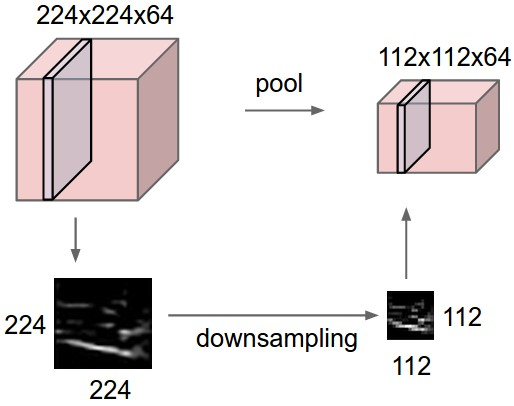
\includegraphics[trim={0cm 0cm 0cm 0cm},clip,width=0.7\linewidth]{Figures/pool.jpeg}
\centering
\caption{A visualization of the down-sampling process using pooling}
\label{pool}
\end{figure}

A pooling layer is commonly inserted in-between successive convolution layers in a CNN architecture. Its main function is to progressively reduce the spatial size of the representation, which in turn reduces the amount of parameters and computation in the network as shown in Figure \ref{pool}. This can be used to control over-fitting. 

\begin{figure}[ht]
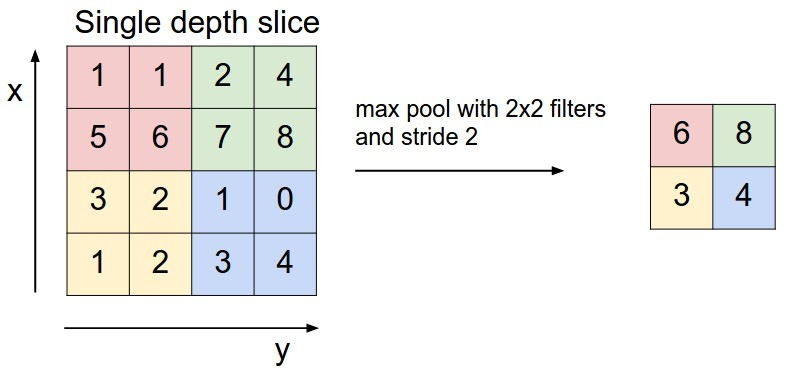
\includegraphics[trim={0cm 0cm 0cm 0cm},clip,width=\linewidth]{Figures/maxpool.jpeg}
\centering
\caption{A visualization of the pooling process}
\label{maxpool}
\end{figure}
Every depth slice of the input is processed independently and spatially resized by the pooling Layer. Pooling is usually done using the MAX operation, however, it is possible to use there operations such as averaging. A pooling layer with filters of size 2x2 applied with a stride of 2 is the most commonly used. As a result, every depth slice in the input is down-sampled by 2 along both width and height. The depth dimension remains unchanged.

\subsubsection{Fully-Connected Layer}
As previously mentioned, each neuron in a fully-connected layer is connected to all activations in the previous layer. Accordingly, computing the activations is a straight-forward matrix multiplication followed by a bias offset. 


\subsection{Visual Geometry Group (VGG)}
\begin{figure}[ht]
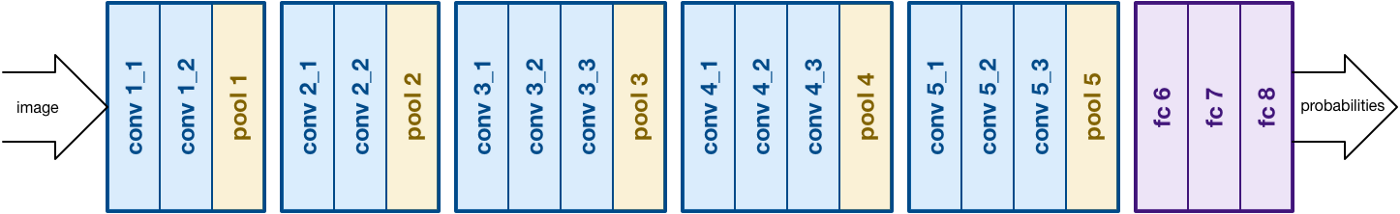
\includegraphics[trim={0cm 0cm 0cm 0cm},clip,width=\linewidth]{Figures/vgg.jpeg}
\centering
\caption{VGG network architecture}
\label{vgg}
\end{figure}
VGG network is characterized by its simplicity, using only 3×3 convolution layers, with 13 stacked layers on top of each other in increasing depth. Reducing volume size is handled by max pooling. Three fully-connected layers, followed by a softmax classifier as shown in Figure \ref{vgg}. It is currently the most preferred choice in the community for extracting features from images. Its main contribution was in highlighting the criticality of the depth of the network and its effect on the network's performance. The network is composed 16 convolution and fully-connected layers. Additionally, the architecture is very homogeneous as the network performs 3x3 convolutions and 2x2 pooling throughout the whole pipeline. A pretrained model is available for plug and play use in Caffe and Keras. \cite{vgg}





% \section{Computer Vision}
\section{Related Work}
Vehicle control systems are the main building blocks for all intelligent vehicle systems and automated driving technologies. The design and implementation of steering and speed controllers are essential for achieving trajectory following for an autonomous vehicle. 

The simplest and most popular form of lateral control algorithm found in the market as well as the literature is the PID (proportional-integral-derivative) controller\cite{pid}. In such controller, the difference between the desired path and the current vehicle state is fed into the controller as the cross-track error. The controller outputs the needed steering actuation command to minimize this error, correcting the vehicle's trajectory, and the next error value is fed back again into the controller.

Recent advancements in the computation capabilities of on-board vehicle control units have made it possible for real-time non-linear model predictive control (NLMPC) to be applied in vehicle lateral and longitudinal control. The predictive behavior of the MPC, along with known vehicle-road dynamics, have given the MPC the possibility to account for the information and obstacles that are ahead of the current vehicle position\cite{mpc}. All this has made the MPC the most popular method for vehicle control.

A different approach to the problem was introduced in a recent study by Nvidia \cite{nvidia}, the well known Graphical Processing Units Manufacturer, which involves the integration of Deep Neural Networks into the autonomous vehicle control field. Their proposed approach is to train a Deep Convolution Neural Network to learn the behavior of the whole processing pipeline that is needed for steering angle prediction of an autonomous vehicle. Based on this description, their approach is referred to as End-to-End deep learning for self-driving cars, where a front-camera is attached to the vehicle, and the system uses only the raw data from this camera (RGB image) to predict the correct steering angle for this particular situation. Their primary motivation was to remove the dependency on specific human-designated features, such as lane markings, road boundaries, or other traffic agents, as well as avoiding traditional rule-based methods that are based on such observed features. End-to-End driving systems date back to 1989, when Pomerleau built \(A\)n \(A\)utonomous \(L\)and \(V\)ehicle \(I\)n a \(N\)eural \(N\)etwork (ALVINN) \cite{alvinn} which was built on a 3-layer back-propagation network that receives as an input images from a front-camera and a laser range finder, and predicts the correct steering angle for following the road ahead. A similar approach was also introduced in 2004 in a project supported by the Defense Advanced Research Projects Agency (DARPA) \cite{dave}. The DARPA Autonomous Vehicle (DAVE) was able to drive through a junk-filled alley. Training was done on a data set of human driving in environments that are similar to the testing track.

Several studies have considered investigating the operation of a convolution neural network to build clear understanding of its performance and potential aspects of improvements\cite{viz}. Complimenting the End-to-End driving study by Nvidia is another study \cite{nvidia_activ} \cite{visualbackprop} that investigated what their above mentioned network learns and how its decisions can be explained and interpreted. They have visualized road features in an image that are of high significance and contribution to the final steering decision of the network.

The purpose of this study is to implement the above mentioned approaches and test them in a variable-free simulation environment. The results are finally plotted, compared and evaluated using relevant performance indicators. Neural Network activations are also visualized to provide an explanation of the networks performance.

%\let\cleardoublepage\clearpage